\documentclass[a4paper, 14pt]{extreport}
\usepackage[T2A]{fontenc}
\usepackage[utf8]{inputenc}
\usepackage[english, russian]{babel}
\usepackage{indentfirst, setspace, titlesec, subcaption}
\usepackage{hyperref}
\usepackage{graphicx}
\usepackage{tocloft}
\usepackage{multirow}
\usepackage[left=2.5cm, right=1.5cm, top=2.0cm, bottom=2.0cm]{geometry}

\graphicspath{{images/}}
\renewcommand{\rmdefault}{ftm}

\titleformat{\chapter}
    {\normalsize}
    {\thechapter}{1em}{}
\titleformat{\section}
    {\normalsize}
    {\thesection}{1em}{}
\titlespacing*{\chapter}{\parindent}{-30pt}{*2}
\titlespacing*{\paragraph}{\parindent}{-30pt}{*2}
\titlespacing*{\section}{\parindent}{*2}{*2}

\renewcommand{\cfttoctitlefont}{\normalfont\hspace{0.38\textwidth}}
\renewcommand{\cftchapleader}{\cftdotfill{\cftdotsep}}
\renewcommand{\cftbeforepartskip}{0em}
\renewcommand{\cftbeforechapskip}{0em}
\renewcommand{\cftchapfont}{\hspace{15pt}\normalsize}
\renewcommand{\cftsecfont}{\hspace{-6pt}}
\renewcommand{\cftsubsecfont}{\hspace{-38pt}}
\renewcommand{\cftchappagefont}{\normalfont}
\renewcommand{\cftbeforetoctitleskip}{-1em}
\renewcommand{\cftpartaftersnumb}{}
\renewcommand{\cftparskip}{-1mm}
\renewcommand{\cftdotsep}{2}

\begin{document}
    \begin{titlepage}
        \begin{center}
            Министерство образования и науки РФ \\
            Государственное образовательное учреждение\\
            Высшего профессионального образования\\
            <<Волгоградский государственный технический университет>>\\
            Кафедра <<САПР~и~ПК>>
        \end{center}
        \vspace{2.0cm}
        \begin{center}
            \large \textbf{ОТЧЁТ} \\
            по преддипломной практике \the\year г.
        \end{center}
        \begin{flushleft}
            Студента\\
            Фамилия \underline{Голубева\hspace{3.1cm}} 
            Имя \underline{Алексея\hspace{2.1cm}}\\
            Отчество \underline{Владимировича\hspace{1.6cm}}\\
            Факультет \underline{ФЭВТ\hspace{3.45cm}} курс \underline{2\hspace{1.5cm}} 
            группа \underline{САПР-2.1п\hspace{1.9cm}}\\
        \end{flushleft}
        \vspace{1.0cm}
        \noindentИндивидуальное задание: \underline{\hspace{22.3em}}\\
        \underline{\hspace{\textwidth}}
        \underline{\hspace{\textwidth}}
        \underline{\hspace{\textwidth}}
        \underline{\hspace{\textwidth}}
        \vspace{2.0cm}
        \begin{flushleft}
            РУКОВОДИТЕЛЬ\\
            Кафедра \underline{САПР~и~ПК\hspace{2.4cm}} Должность \underline{профессор\hspace{2.8cm}} \\
            Фамилия \underline{Кравец\hspace{3.3cm}} Имя \underline{Алла\hspace{5.5cm}}\\
            Отчество \underline{Григорьевна\hspace{2.2cm}}
        \end{flushleft}
        \vspace{1.5cm}
        \begin{flushright}
            <<\underline{\hspace{1.0cm}}>>\underline{\hspace{4.0cm}} \the\year г.
        \end{flushright}
        \vspace{\fill}
        \begin{center}
            Волгоград \the\year
        \end{center}
    \end{titlepage}
    \tableofcontents
    \onehalfspacing

    \chapter{Разработка методик тестирования системы построения маршрутов}
    Алгоритмы предложенные в рамках магистерской работы были реализованы с использованием языка программирования 
    Python и сервиса построения маршрутов Open Source Routing Machine (OSRM) для расчёта расстояния между узлами графа 
    по городским дорогам. Программный код опубликован на хостинге Github 
    \url{https://github.com/vstu-cad-stuff/routing/tree/master}.

    Для оценки эффективности алгоритма и изучения его специфики, были проведены эксперименты в ходе которых менялось 
    количество узлов в дорожном графе и количество создаваемых маршрутов в городской сети, а также несколько вариантов 
    реализации данного метода. Наиболее интересным случаем является, когда обрабатывается большое число узлов в графе 
    или большое число геопространственных данных.

    Были сгенерированы данных о предпочтениях по перемещению жителей среднего по размерам города с примерным числом 
    жителей около 350 000. В качестве результата, было получено 6000 пар точек отправления-назначения или 12000 точек в 
    общей сложности. Матрица корреспонденций в данном случае имеет очень большой размер \( 6000 \times 6000 \) 
    элементов, где элемент с индексом \( i, j \) имеет значение \( 0 \) -- отсутствие связи между \( i \)-ой и 
    \( j \)-ой точкой, а \( 1 \) соответственно связь.

    Для того, чтобы уменьшить размер матрицы корреспонденций и понять наиболее густонаселённые места, был применён 
    алгоритм кластеризации точек отправления-назначения, который не входит в рассмотрение в данной работе.

    Для получения понимания какое количество кластеров (или узлов) влияет на эффективность работы предложенного 
    алгоритма было предложено произвести варьирование параметров: количество кластеров и количество маршрутов для 
    построения.

    \chapter{Произведение испытаний разработанной системы}
    По мере того как количество кластеров изменяется получаем различные варианты производительности алгоритма. В 
    проводимых экспериментах число узлов изменяется в диапазоне от 100 до 300.

    Количество маршрутов для построения так же влияет на скорость работы предложенного алгоритма. Очевидно, что 
    минимальное количество маршрутов определяется числом пар терминальных маршрутов. В данном случае варьирование числа 
    маршрутов было произведено в интервале от 8 до 100 в зависимости от количества узлов.

    В эксперименте использовалось эмпирическое правило, что число узлов должно быть в 20 раз больше, чем число 
    маршрутов. Для упрощения оценки производительности применяется общая длина сети в качестве критерия качества.
    Поскольку эта оценка производится во внешнем цикле, то она не имеет большого влияния на выполнение алгоритма. Кроме 
    того не была использована информация о возможных пробках влияющая на процедуру выбора соответствующего узла.

    Чтобы понять эффективность работы алгоритма в зависимости от окружающей среды, были разработаны три альтернативных 
    реализации:
    \begin{enumerate}
        \item Последовательная реализация (или graph) алгоритма основанного на графе дорог. В данной реализации 
            предполагается, что связь между узлами может быть проведена по прямой линии, несмотря на состояние 
            дорог. Эту реализацию можно рассматривать в качестве базовой.
        \item Последовательная реализация с использованием OSRM (или S.OSRM) -- это усовершенствованная версия 
            предыдущей стратегии, где расстояние между кластерами рассчитывается с использование движка 
            маршрутизации OSRM по дорожной сети.
        \item Параллельная версия с использованием OSRM (или P.OSRM) предполагает возможность в распараллеливании 
            внутреннего цикла алгоритма.  
    \end{enumerate}

    \chapter{Результаты полученные в входе работы}
    Результаты представлены на рисунках \ref{fig:result-01} и \ref{fig:result-02}, а также в таблице 
    \ref{tab:second_alg}. Рисунки представлены в логарифмической шкале по оси ординат, для более удобного 
    анализа данных.

    \begin{figure}[ht!]
        \centering
        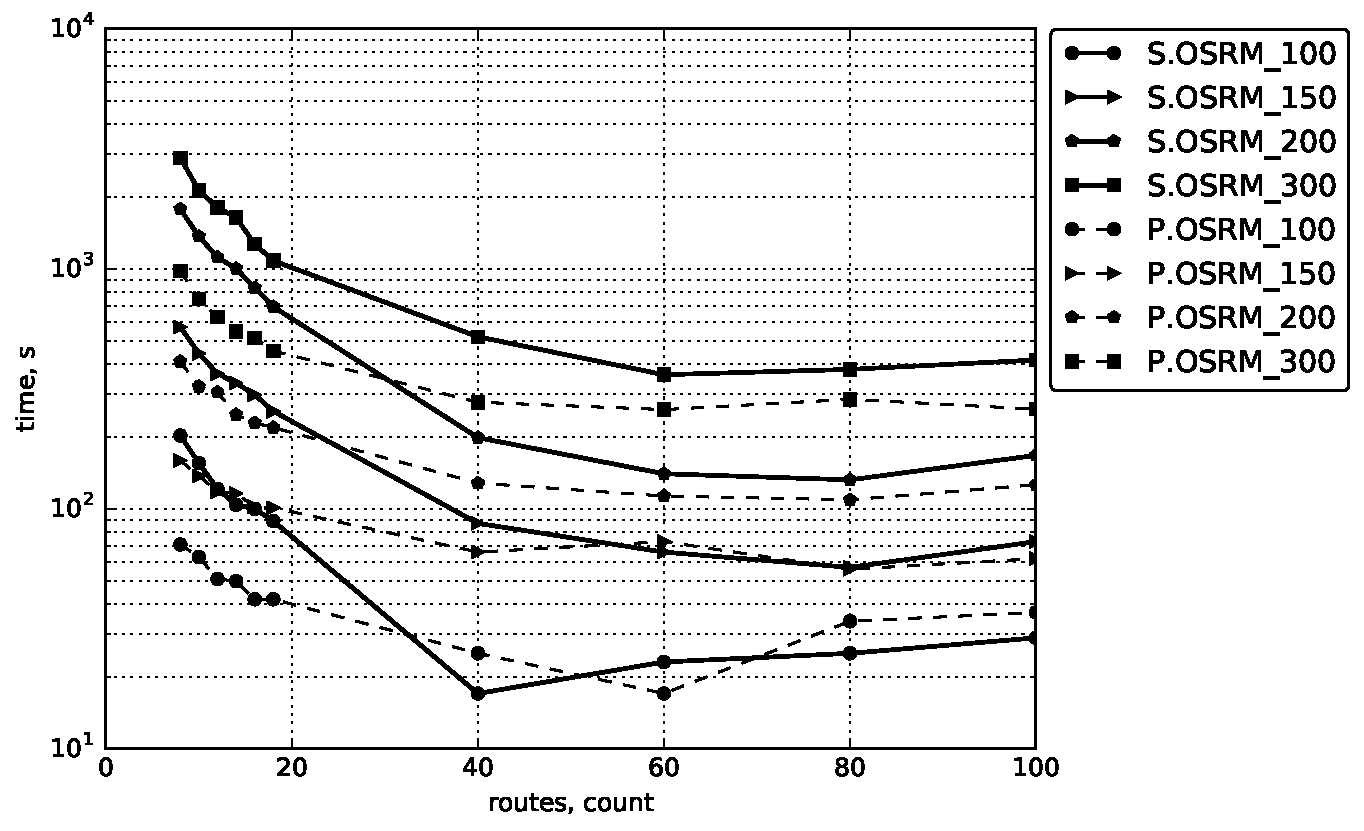
\includegraphics[width=0.9\textwidth]{result-01}
        \caption{Зависимость времени построения от количества маршрутов}
        \label{fig:result-01}
    \end{figure}

    \begin{figure}[ht!]
        \centering
        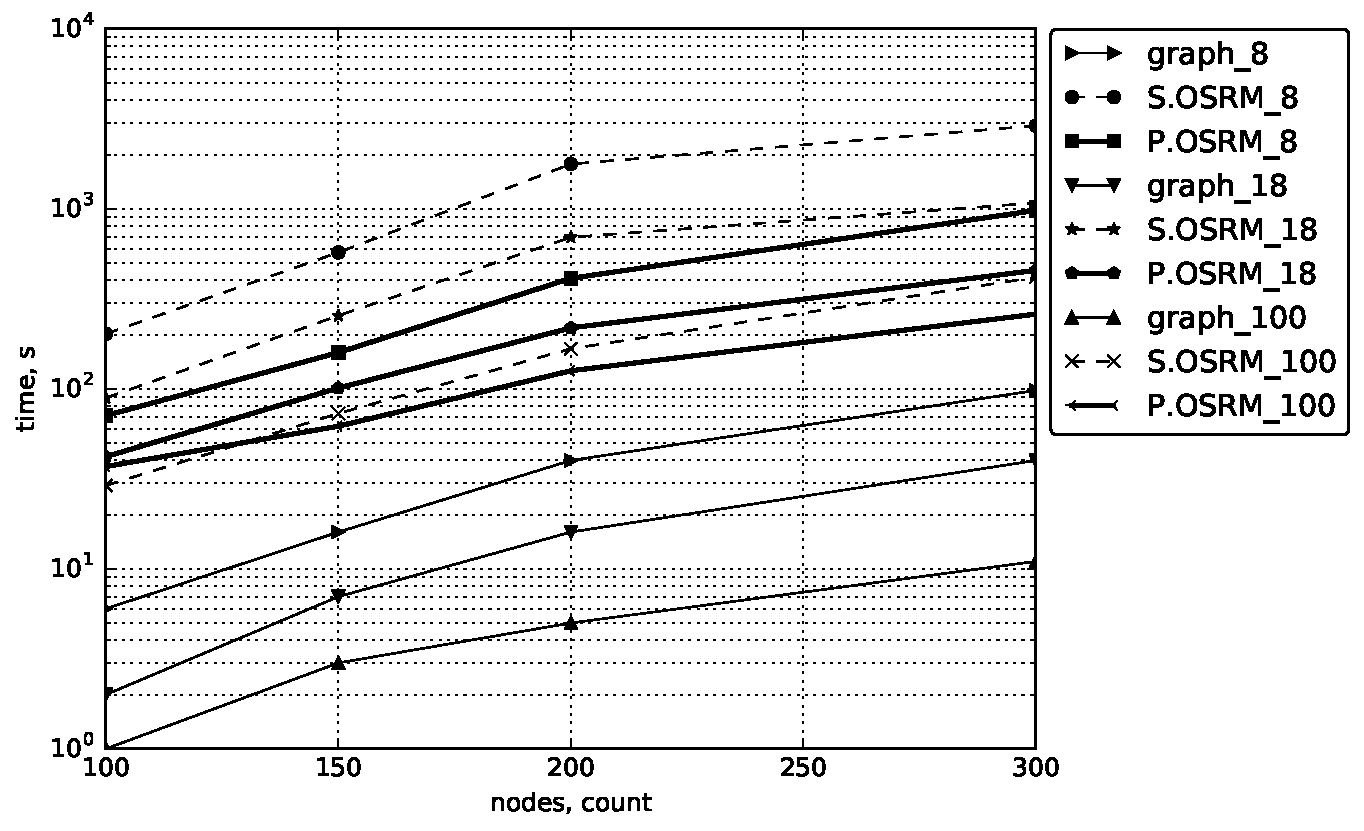
\includegraphics[width=0.9\textwidth]{result-02}
        \caption{Зависимость времени построения от кластеров}
        \label{fig:result-02}
    \end{figure}

    \begin{figure}[ht!]
        \centering
        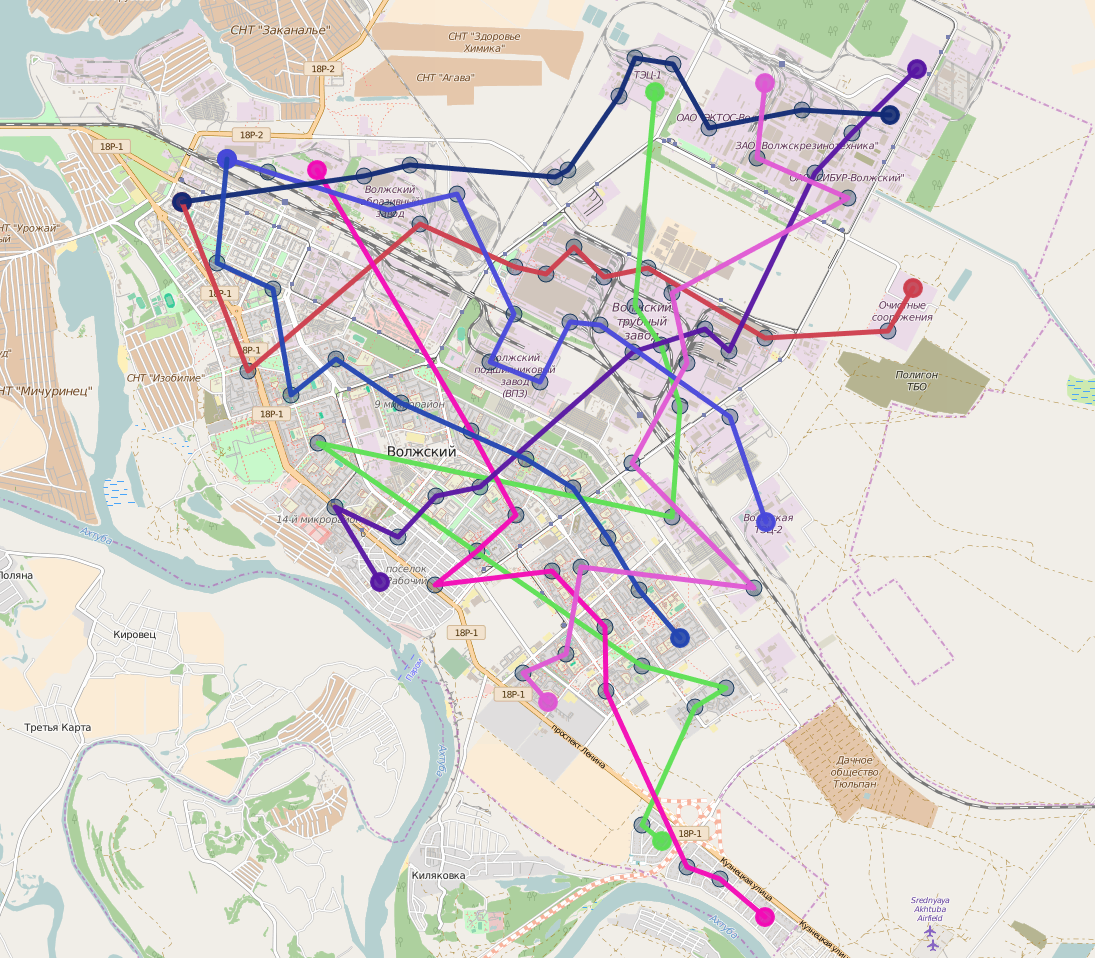
\includegraphics[width=0.75\textwidth]{minimal-01}
        \caption{Использование метрики graph для 100 кластеров и 8 маршрутов.}
        \label{fig:network-01}
    \end{figure}

    \begin{figure}[ht!]
        \centering
        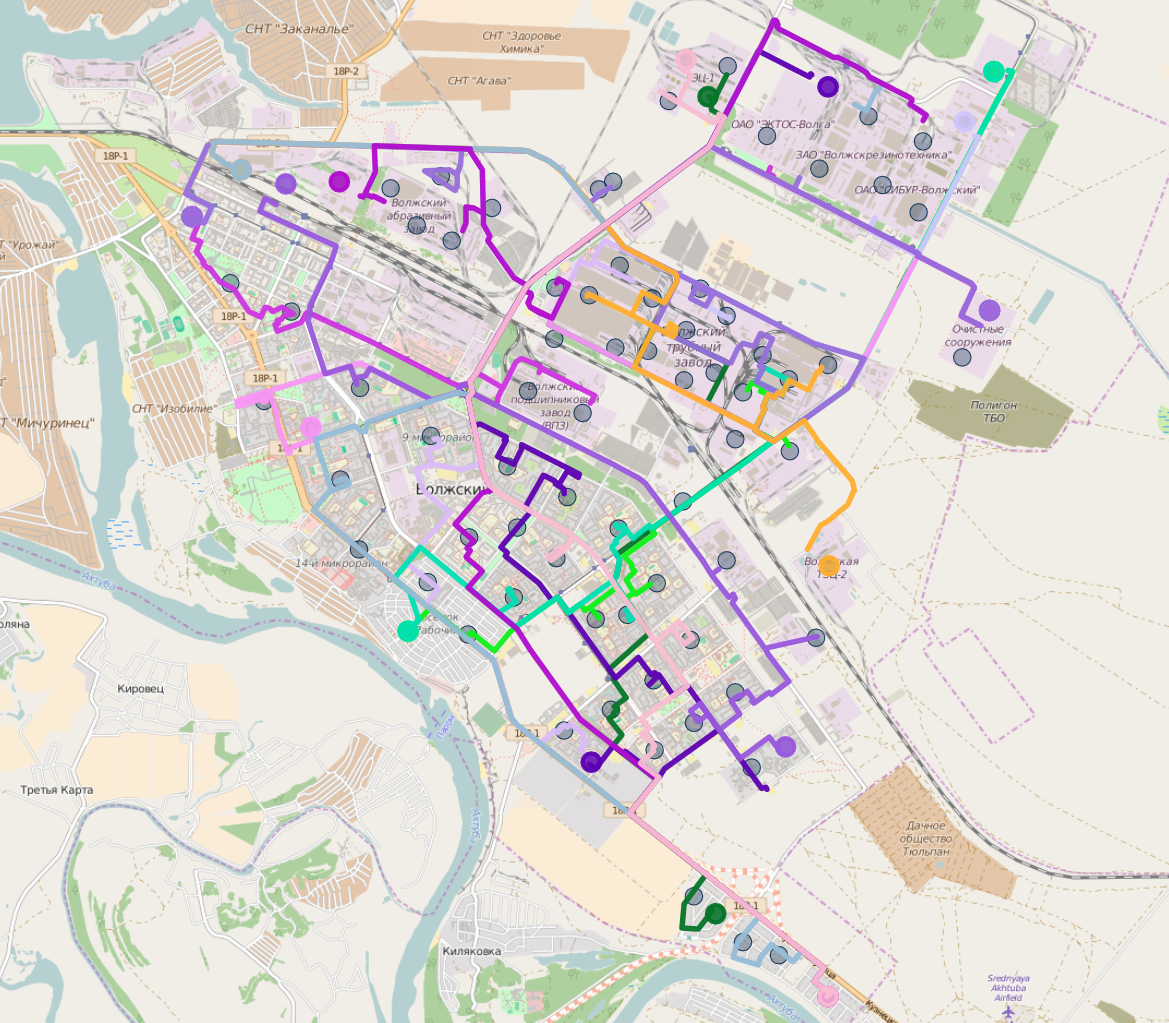
\includegraphics[width=0.75\textwidth]{minimal-02}
        \caption{Использование метрики OSRM для 100 кластеров и 14 маршрутов.}
        \label{fig:network-02}
    \end{figure}

    \newpage

    \begin{table}[ht!]
        \centering
        \caption{Результаты эксперимента алгоритма минимального увеличения длины маршрута. Данные представлены в 
            формате минуты:секунды.}
        \label{tab:second_alg}
        \small
        \begin{tabular}{|c|l|c|c|c|c|c|c|l|l|l|c|}
            \hline
            \multicolumn{1}{|l|}{}      &          & \multicolumn{10}{c|}{routes}                                                                                                       \\ \hline
            \multicolumn{1}{|l|}{nodes} & strategy & 8     & 10    & 12    & 14    & 16    & 18    & \multicolumn{1}{c|}{40} & \multicolumn{1}{c|}{60} & \multicolumn{1}{c|}{80} & 100  \\ \hline
            \multirow{3}{*}{100}        & graph    & 0:06  & 0:04  & 0:03  & 0:03  & 0:02  & 0:02  & 0:01                    & 0:01                    & 0:01                    & 0:01 \\ \cline{2-12} 
            & S. OSRM  & 3:22  & 2:35  & 2:01  & 1:44  & 1:40  & 1:29  & 0:17                    & 0:23                    & 0:25                    & 0:29 \\ \cline{2-12} 
            & P. OSRM  & 1:11  & 1:03  & 0:51  & 0:50  & 0:42  & 0:42  & 0:25                    & 0:17                    & 0:34                    & 0:37 \\ \hline
            \multirow{3}{*}{150}        & graph    & 0:16  & 0:12  & 0:10  & 0:08  & 0:07  & 0:07  & 0:04                    & 0:03                    & 0:02                    & 0:03 \\ \cline{2-12} 
            & S. OSRM  & 9:32  & 7:24  & 6:06  & 5:34  & 4:59  & 4:15  & 1:27                    & 1:06                    & 0:57                    & 1:13 \\ \cline{2-12} 
            & P. OSRM  & 2:39  & 2:17  & 1:58  & 1:56  & 1:42  & 1:41  & 1:06                    & 1:13                    & 0:56                    & 1:02 \\ \hline
            \multirow{3}{*}{200}        & graph    & 0:40  & 0:31  & 0:25  & 0:20  & 0:20  & 0:16  & 0:08                    & 0:06                    & 0:05                    & 0:05 \\ \cline{2-12} 
            & S. OSRM  & 29:33 & 22:45 & 18:36 & 16:43 & 13:53 & 11:35 & 3:18                    & 2:20                    & 2:12                    & 2:47 \\ \cline{2-12} 
            & P. OSRM  & 6:51  & 5:23  & 5:06  & 4:07  & 3:48  & 3:38  & 2:08                    & 1:53                    & 1:49                    & 2:06 \\ \hline
            \multirow{3}{*}{300}        & graph    & 1:38  & 1:16  & 1:02  & 0:51  & 0:46  & 0:40  & 0:20                    & 0:14                    & 0:11                    & 0:11 \\ \cline{2-12} 
            & S. OSRM  & 48:20 & 35:24 & 30:00 & 27:17 & 21:06 & 18:01 & 8:41                    & 6:02                    & 6:21                    & 6:57 \\ \cline{2-12} 
            & P. OSRM  & 16:20 & 12:28 & 10:31 & 9:08  & 8:35  & 7:35  & 4:38                    & 4:19                    & 4:46                    & 4:20 \\ \hline
        \end{tabular}
    \end{table}

    \chapter{Структура четвёртой главы магистерской диссертации}
    В структуре четвёртой главый магистерской диссертации были выделены следующие пункты:
    \begin{enumerate}
        \item Испытание и обоснование эффективности предлагаемых подходов
        \begin{enumerate}
            \item Проектирование ПО
            \item Методика проведения эксперимента
        \end{enumerate}
        \item Методология и результаты
        \begin{enumerate}
            \item Проведение эксперимента и описание результатов
            \begin{enumerate}
                \item Последовательная реализация
                \item Последовательная с использованием OSRM
                \item Параллельная с использованием OSRM
                \item Результаты
            \end{enumerate}
            \item Обсуждение результатов
            \item Заключение
        \end{enumerate}
    \end{enumerate}

    В разделе <<Испытание и обоснование эффективности предлагаемых подходов>> описана методика тестирования 
    разработанных алгоритмов и данные используемые для проведения тестирования.

    В разделе <<Методология и результаты>> были предложены три альтернативных реализации алгоритма, для оценки его 
    эффективности, в зависимости от входных данных. В данном разделе производится оценка эффективности альтернативных 
    реализаций и их общее сравнение. Результатом работы является графики быстродействия данных реализаций представленные 
    на рисунках \ref{fig:result-01} и \ref{fig:result-02}, а также в таблице \ref{tab:second_alg}.

    \chapter{Выводы по проделанной работе}
    В ходе преддипломной практики были выполнены следующие задачи:
    \begin{itemize}
        \item разработана методика тестирования системы построения маршрутной сети общественного транспорта на 
            основании обработки данных;
        \item произведены испытания разработанной системы построения маршрутной сети общественного транспорта на 
            тестовом наборе входных данных;
        \item произведена оценка построенных маршрутных сетей по критериям эффективности (суммарная длина маршрутной 
            сети, пассажиропоток и д.р.) и обоснована эффективность используемых алгоритмов.
    \end{itemize}

    \chapter{Используемые технологии в работе}
    Для проектирования и вёрстки были использованы следующие свободно распространяемые программные 
    продукты:
    \begin{itemize}
        \item Arch Linux -- это независимо разрабатываемый i686/x86-64 дистрибутив GNU/Linux общего 
            назначения \url{https://www.archlinux.org/}
        \item \TeX -- система компьютерной вёрстки, разработанная американским профессором информатики 
            Дональдом Кнутом в целях создания компьютерной типографии. \url{http://tug.org/}
        \item \LaTeX -- набор макрорасширений системы компьютерной вёрстки TeX.\\
            \url{http://www.latex-project.org/}
        \item Atom -- свободный открытый текстовой редактор исходных текстов программ.
            \url{https://atom.io/}
        \item Python -- высокоуровневый язык программирования общего назначения, ориентированный на повышение 
            производительности разработчика и читаемости кода. \url{https://www.python.org/}
        \item Matplotlib -- библиотека на языке программирования Python предназначенная для визуализации данных.
            \url{http://matplotlib.org/}
        \item Git -- распределённая система управления версиями файлов. Проект был создан Линусом 
            Торвальдсом для управления разработкой ядра Linux, первая версия выпущена 7 апреля 2005 года.\\
            \url{http://git-scm.com/}
        \item GitHub -- самый крупный веб-сервис для хостинга IT-проектов и их совместной разработки. 
            Основан на системе контроля версий Git и разработан на Ruby on Rails и Erlang компанией 
            GitHub, Inc.\\ \url{https://github.com/}
    \end{itemize}
\end{document}